\documentclass{beamer}
\usepackage{tikz}
\usepackage{svg}
\usepackage{mwe}
\usepackage[off]{svg-extract}
\usetikzlibrary{calc}
\usetikzlibrary{arrows.meta}
\title{Scientific Programming in C++}
% TODO: subtitle
% TODO: understand how to make slides collapse and how they do not collapse - we did this before I strongly remember
\author{Bram Kuijper}
%\titlegraphic{\includesvg[width=\textwidth,height=.5\textheight]{img/iso\_cplusplus\_logo}}
\date{}
\begin{document}
\begin{frame}
\titlepage
    \vspace{-.2\textheight}
    \begin{center}
    \includesvg[width=\textwidth,height=.3\textheight]{isoCPPLogo}
    \end{center}
\end{frame}
\begin{frame}{Aims of this course}
    \begin{columns}
        \begin{column}{0.5\textwidth}
            \begin{enumerate}
                \item<1-> Develop C++ programs for scientific purposes
                \item<2-> Do so on Linux-based high-performance computing environments (HPCs) 
                \item<3-> Detect, analyse and solve coding errors
                \item<4-> Evaluate code performance
                \item<5-> Interpret C++ documentation and use this to aquire new knowledge 
            \end{enumerate}
        \end{column}
        \begin{column}{0.5\textwidth}
            \begin{figure}
                \only<2>{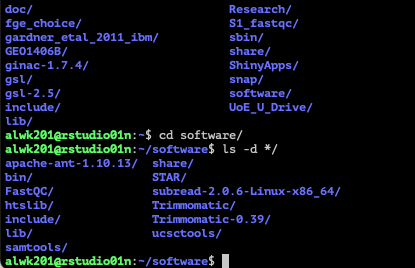
\includegraphics[width=0.8\textwidth]{img/commandLine}}%
                \only<3>{
\includegraphics[width=0.8\textwidth]{img/segfault}}%
                \only<4>{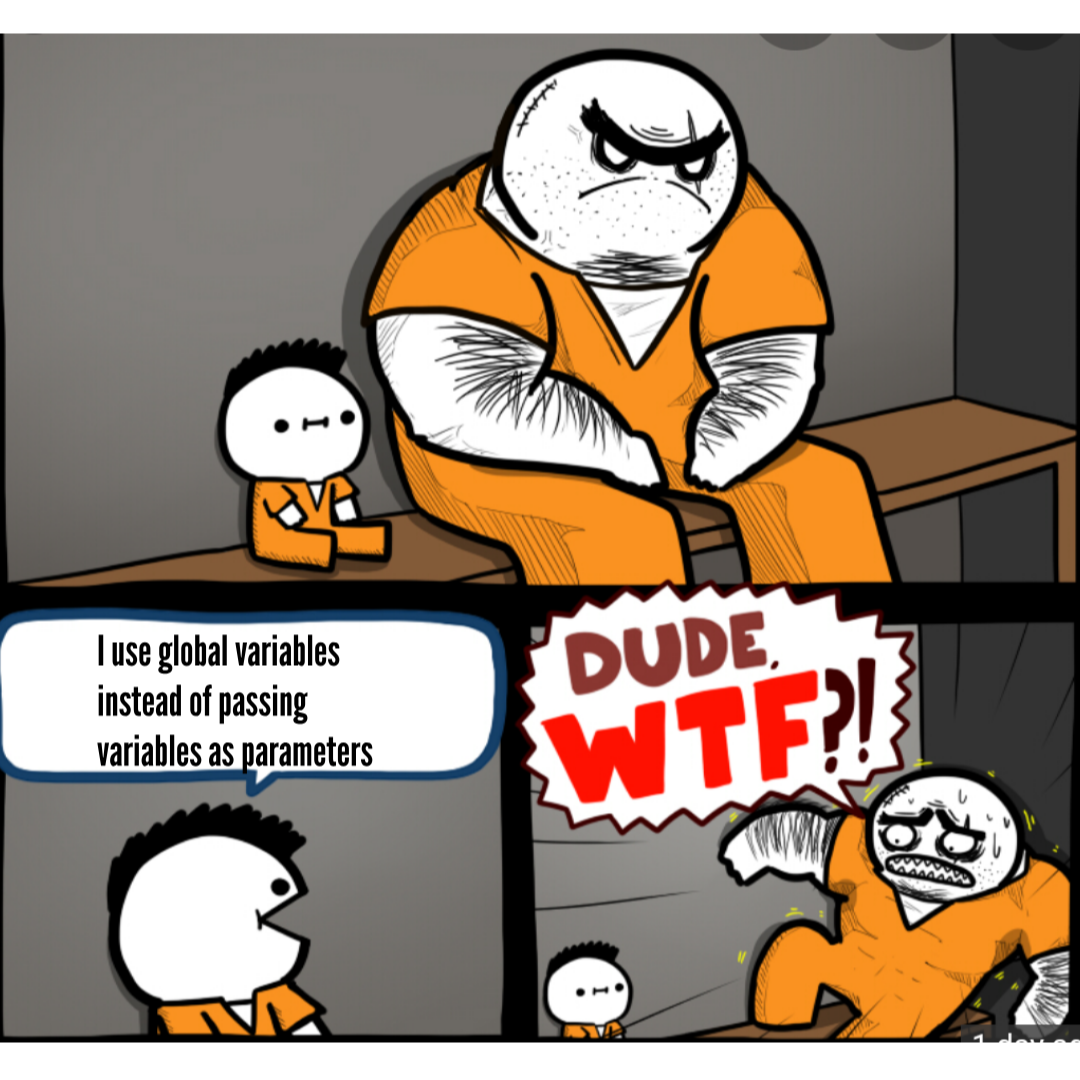
\includegraphics[width=0.8\textwidth]{img/dude.png}}
                \only<5>{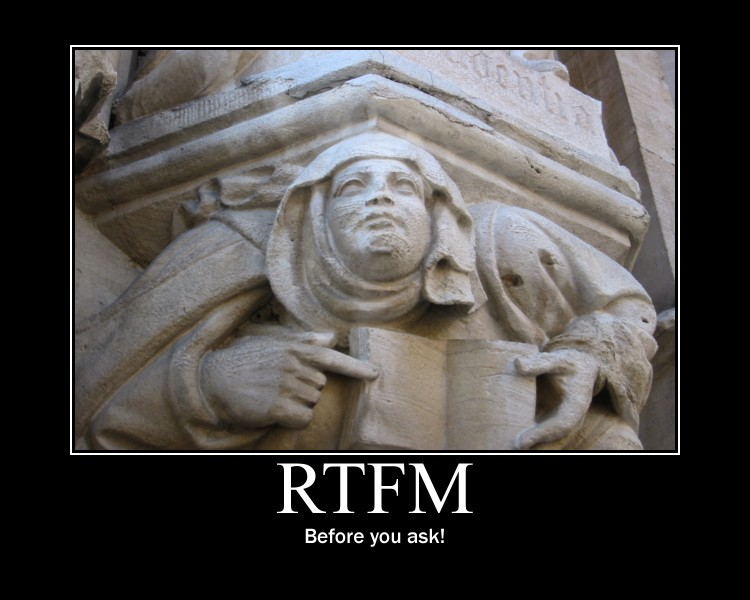
\includegraphics[width=0.8\textwidth]{img/rtfm.jpg}}
            \end{figure}
        \end{column}
    \end{columns}
\end{frame}
\begin{frame}{Outline of this lecture}
    \begin{enumerate}
        \item Aims of this course \checkmark
            \pause
        \item Understand what C++ is and how it differs from other programming languages 
            \pause
        \item How to \emph{learn} during this course?
            \pause
        \item An overview of documentation and other resources
            \pause
        \item The programming environment: the Linux shell, \texttt{SSH}, \texttt{g++} and text editors
    \end{enumerate}
\end{frame}
\begin{frame}{What is C++}
    \begin{columns}
        \begin{column}{0.5\textwidth}
            \begin{itemize}
                \item<2-> It is a superset of the C programming language
                    \begin{itemize}
                        \item If you know C++, relatively easy to learn C too 
                        \item Allows you to use C libraries within C++
                    \end{itemize}
                \item<3-> C++ focuses on applications in which resources are limiting...
                    \begin{itemize}
                        \item Resources you say? Speed and memory
                    \end{itemize}
                \item<4-> ... at the expense of a longer development time
                    \begin{itemize}
                        \item Writing a program in Python will be faster (but will run slower)
                    \end{itemize}
            \end{itemize}
        \end{column}
        \begin{column}{0.5\textwidth}
            \begin{figure}
                \only<2>{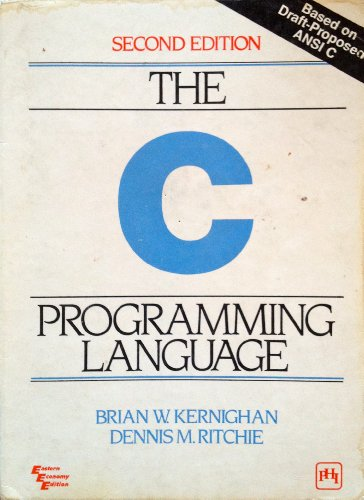
\includegraphics[width=0.8\textwidth]{img/kerniganritchie.jpg}}%
            \end{figure}
        \end{column}
    \end{columns}
\end{frame}
\begin{frame}{What is C++ (continued)}
    \begin{columns}
        \begin{column}{0.5\textwidth}
            \begin{itemize}
                \item<1-> Examples of software written in C++
                    \begin{itemize}
                        \item Desktop applications like Microsoft Office, Adobe Photoshop
                        \item Major scientific libraries like Eigen, STAN, GDAL
                    \end{itemize}
                \item<2-> \#3 or \#4 of the most frequently used languages worldwide
                    \begin{itemize}
                        \item \href{https://www.tiobe.com/tiobe-index/}{TIOBE index}
                    \end{itemize}
            \end{itemize}
        \end{column}
        \begin{column}{0.5\textwidth}
            \begin{figure}
                \only<2>{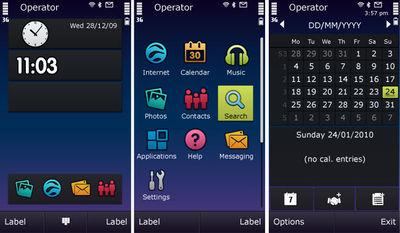
\includegraphics[width=0.8\textwidth]{img/symbian.jpg}}%
            \end{figure}
        \end{column}
    \end{columns}
\end{frame}


\begin{frame}{Interpreted languages vs compiled languages}
    C++ is a compiled language, whereas Python, R, Javascript typically$^*$ use an interpreter
\begin{center}
    
\begin{tikzpicture}
[>=latex]
    \draw[line width=1.5mm,white!50!black, ->] (-3,0) -- (-3,-1);
    \visible<2->{%
[>=latex]
    \draw[line width=1.5mm,white!50!black, ->] (0,0) -- (0,-1);
    }
    \end{tikzpicture}
\end{center}
\end{frame}
\end{document}
